\documentclass{beamer}

\usepackage[utf8]{inputenc}
\usepackage{eurosym}
\usepackage{hyperref}
\hypersetup{
    colorlinks = true
    }
\usepackage{graphicx}

%Information to be included in the title page:
\title{GTA Einführung Robotik mit Makecode}
\author{Mattias Schlenker}
\institute{Wilhelm-Ostwald-Gymnasium}
\date{7. Januar 2021}

\begin{document}

\frame{\titlepage}

\begin{frame}
\frametitle{Wir verbessern den Space-Shooter}

Viele von uns haben am Shooter weiter programmiert, daher gab es einige Fragen zu Spielmechanik, aber auch Fehlersuche und ,,Best Practices'' hinsichtlich Übersichtlichkeit. Wichtig: Wir haben uns die Funktion der Kollisionserkennung noch einmal im Detail angesehen.
 
\end{frame}
 
 \begin{frame}
 \frametitle{Pizza!}
 
Neu eingeführt haben wir Versorgungsraumschiffe, die wir der Bequemlichkeit halber mit einem Pizza-Sprite versehen haben und die etwa alle fünf Sekunden erscheinen sollen. Maßgabe war, dass fünf Pizza-Sprites ein neues Leben ergeben. Für die Pizza-Sprites haben wir eine neue Kategorie ,,Food'' eingeführt:
 
 \begin{figure}
  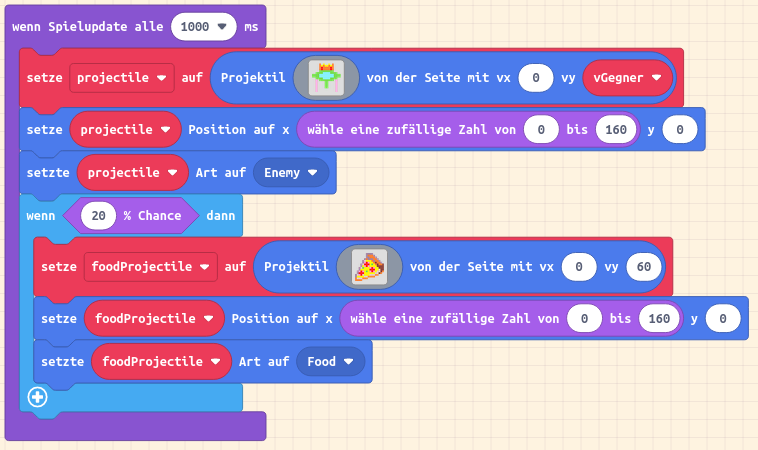
\includegraphics[width=8cm]{game15.png}
  \caption{Pizza!}
  \label{fig:game15}
\end{figure}

\end{frame}

 \begin{frame}
 \frametitle{Protokollierung}
 
Viele Entwicklungsumgebungen bieten die Möglichkeit, Werte oder Text zu protokollieren. Das nennt sich ,,Debugging-Ausgaben schreiben''. Makecode bietet dafür die Klasse ,,Konsole''. Nutzt sie! Initialisiert eine Variable und schreibt sie nach jeder Änderung auf die Konsole.  
 
 \begin{figure}
  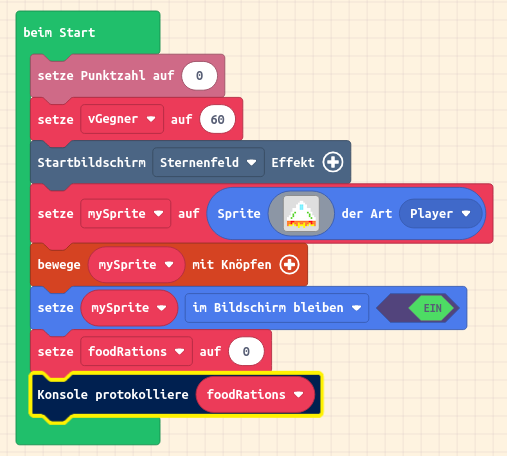
\includegraphics[width=5cm]{game16.png}
  \caption{Konsolen-Logging}
  \label{fig:game16}
\end{figure}

\end{frame}

 \begin{frame}
 \frametitle{Woher kommt das Wort ,,Debugging''}
Ein ,,Bug'' ist ein Käfer, aber was hat der in einem Programm zu suchen? Als die Logikgatter noch Relais (elektromagnetische Schalter) waren, sagten Programmierer gerne: ,,Da ist sicher ein Insekt im Schalter. ICH habe richtig programmiert.'' 1947 wurde tatsächlich mal eine Motte in einem Relais gefunden:  

 
 \begin{figure}
  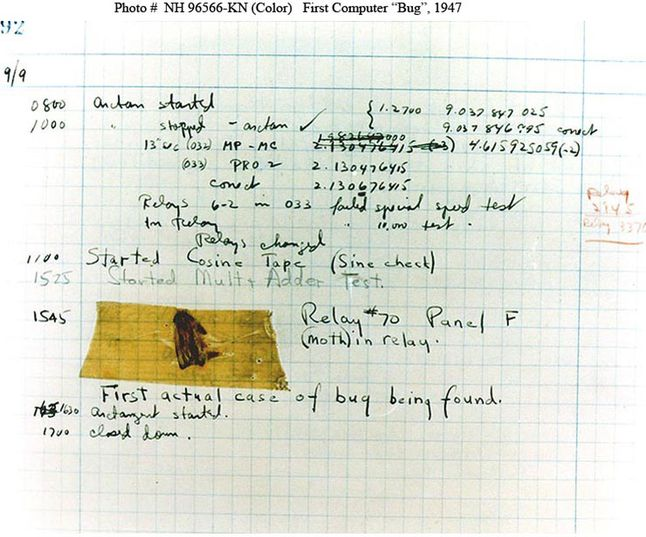
\includegraphics[width=6cm]{debug.jpeg}
  \caption{Debugging}
  \label{fig:debugging}
\end{figure}
\end{frame}

 \begin{frame}
 \frametitle{Konsolenausgabe}
Ihr schaltet die Konsolenausgabe im laufenden Spiel über den Button ,,Konsole anzeigen'' an. 
 
 \begin{figure}
  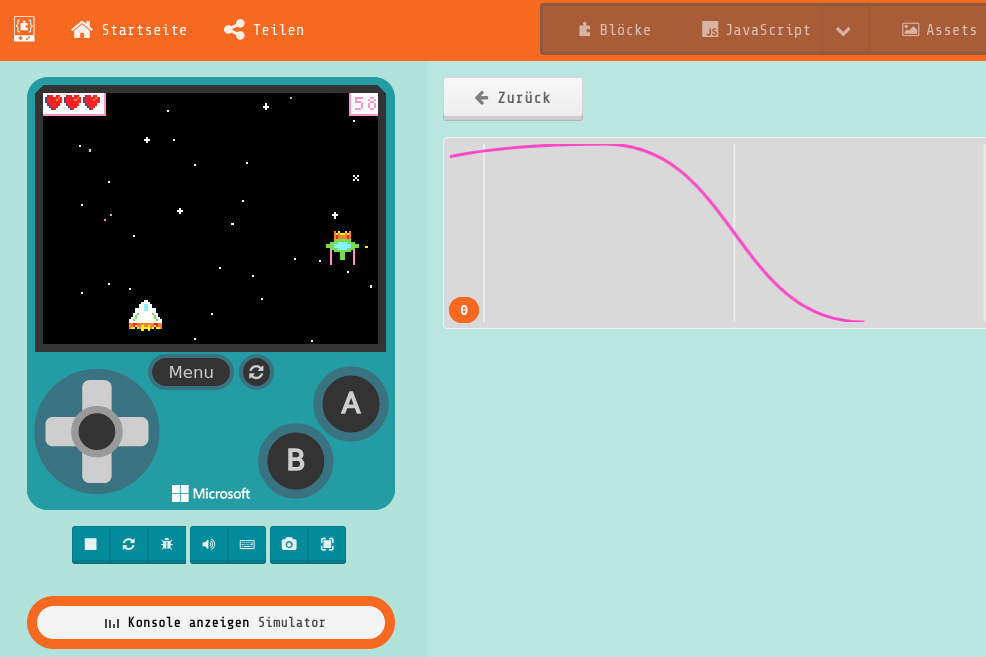
\includegraphics[width=8cm]{game17.png}
  \caption{Debug-Ausgabe}
  \label{fig:game17}
\end{figure}
\end{frame}


 \begin{frame}
 \frametitle{Variablen als Referenzen übergeben}
Wenn ein Sprite mit einem anderen kollidiert, kennen wir deren Namen nicht. Daher wird eine Referenz erzeugt und diese in die Funktion hinein übergeben. Verwendet innerhalb der Funktion nur die Referenzen ,,sprite'' und ,,otherSprite''! 
 
 \begin{figure}
  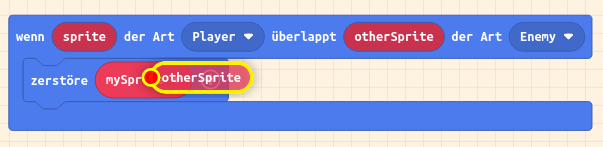
\includegraphics[width=11cm]{game05.png}
  \caption{Kollisionserkennung}
  \label{fig:game5}
\end{figure}
\end{frame}

 \begin{frame}
 \frametitle{Best Practices}

Wie mit einer Vielfalt von Gegnern und Essensrationen umgehen, ohne das Spiel unübersichtlich zu machen?

Nutzt möglichst wenige Blöcke des Typs ,,Spielupdate''. Verwendet stattdessen innerhalb eines Blockes Verzweigungen, die Zufallsvariablen nutzen, um verschiedene Gegner zu spawnen oder gelegentlich mal eine Pizza zu droppen.


\end{frame}


 \begin{frame}
 \frametitle{Spiele weitergeben}
Klickt auf das Diskettensymbol, um das Spiel zu speichern. Die Bild-Datei im PNG-Format enthält einen Screenshot und den Programmcode. Natürlich könnt Ihr auch ,,Herunterladen'' klicken, das erzeugt fertige UF2-Dateien für Spielekonsolen. Und mit ,,Teilen'' erzeugt Ihr einen Link für Mitschüler und mich. 
 
 \begin{figure}
  
\includegraphics[width=13cm]{game18.png}
  \caption{Herunterladen}
  \label{fig:game4}
\end{figure}
\end{frame}

\end{document}
